\documentclass{beamer}
\mode<presentation>
\usepackage{tikz}
\usepackage{graphicx}
\usepackage{tabu}
\usetikzlibrary{positioning}
\usetikzlibrary{calc}
\usefonttheme{professionalfonts}
\usetheme{Orr}
\usepackage[orientation=portrait,width=1m,height=1.2m,scale=1.4]{beamerposter}
\graphicspath{{./figures/}{./figures/generated/}{./figures/static/}}

\title{Patterns of somatic mutation correspond to physical topology in \textit{Eucalyptus}}
\titlegraphic{
	
\includegraphics[width=.95\linewidth]{biodesign_logo.pdf}
	}
\date{4/8/16}
\author{Adam J Orr \inst{1,2} \and Robert Lanfear \inst{3} \and Reed Cartwright \inst{1,2}}
\institute{\inst{1} School of Life Sciences, Arizona State University \\
		   \inst{2} Biodesign Institute, Arizona State University \\
		   \inst{3} College of Medicine, Biology and Environment, Australian National University}
\email{ajorr1@asu.edu}
\website{cartwrig.ht/lab/}

\begin{document}

\begin{frame}{}
\begin{columns}

%%%% Left side %%%%

\column{.5\linewidth}

%%%%%%%%%%%%%%%%%%%

% \begin{block}{\large Abstract}
% \textit{Eucalyptus melliodora}, a tree native to eastern Australia, has strong timber and a high nectar load, making it economically important and a vital source of food for nectar-consuming species. In 1993, an individual of the species was discovered that harbors a somatic change conferring herbivore resistance to a section of branches on the tree via differential terpenoid production. Though transcriptomic analysis was inconclusive in determining the genetic source of this variation, we attempt to do so using ultra-deep whole-genome sequencing of 8 samples in triplicate. We call variants using a reference-free De-Bruijn variant caller \textit{DiscoSNP++} and by the GATK best practices using a reference from a closely-related species. We find that the phylogeny of the variants identified by both methods reflects the branching pattern of the tree, though the phylogeny is affected by short interior nodes. While we have yet to validate the source of the herbivore resistance, this data presents an opportunity for further study of how somatic mutations are produced and spread in plants and how to properly resolve short interior nodes.
% \end{block}


\begin{block}{Introduction}

\begin{itemize}
\item Somatic mutations are rare but sequencing errors are common, making somatic mutations difficult to detect.
\item Little is known about the spread of somatic mutations, despite the key role they play in cancer development.
\item The branching pattern of trees can be used to validate methods for detecting somatic mutations.
\end{itemize}

\end{block}





\begin{block}{Methods: Variant Detection}

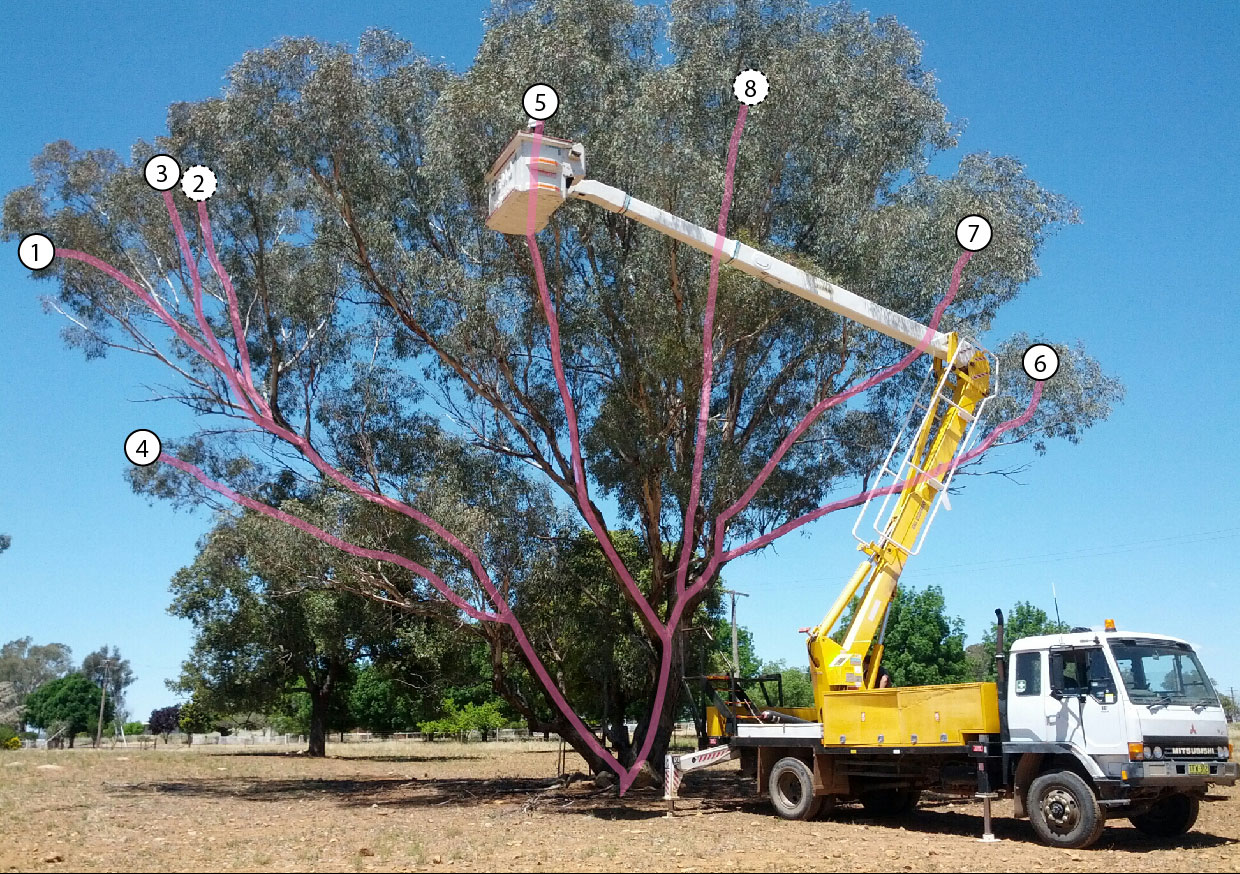
\includegraphics[width=.97\linewidth]{labeled_tree.jpg}

\vskip 2ex

\begin{itemize}
\item 8 samples collected in triplicate
% \item Each replicate was Illumina sequenced
% \item Each sequence was aligned to genome of \textit{Eucalyptus grandis} using bwa mem.
% \item Variants were called using GATK's UnifiedGenotyper or DiscoSNP++, a reference-free variant caller
% \item Nonvariable sites and gaps were removed
\item Variants were removed if the genotypes of all replicates of a sample were not identical
% \item A maximum likelihood tree was constructed with RAxML
\end{itemize}

\vskip 2ex

\begin{center}
	\begin{tikzpicture}[align=center, sqnode/.style={rectangle,draw=black!60,fill=black!5,very thick,minimum size=1cm}]
		\node[sqnode] (sequencing) {Sequence};
		\node[sqnode] (filter) [below = 7cm of sequencing] {Filter};
		\node[sqnode] (alignment) [below left = of sequencing] {Alignment};
		\node[sqnode] (gatk) [above left = of filter] {Get Variants (GATK)};
		\node[sqnode] (discosnp) [above right = of filter] {Get Variants (DiscoSNP++)};
		\node[sqnode] (tree) [below = of filter] {Tree Construction};
		\draw[line width=3mm,->] (sequencing) -- (alignment);
		\draw[line width=3mm,->] (sequencing) -- (discosnp);
		\draw[line width=3mm,->] (alignment) -- (gatk);
		\draw[line width=3mm,->] (gatk) -- (filter);
		\draw[line width=3mm,->] (discosnp) -- (filter);
		\draw[line width=3mm,->] (filter) -- (tree);
	\end{tikzpicture}
\end{center}


\end{block}

\begin{block}{Results: Variant Detection}

\vskip 1ex

% \begin{columns}
% 	\column{.4\linewidth}
% 	\begin{block}{GATK}
% 	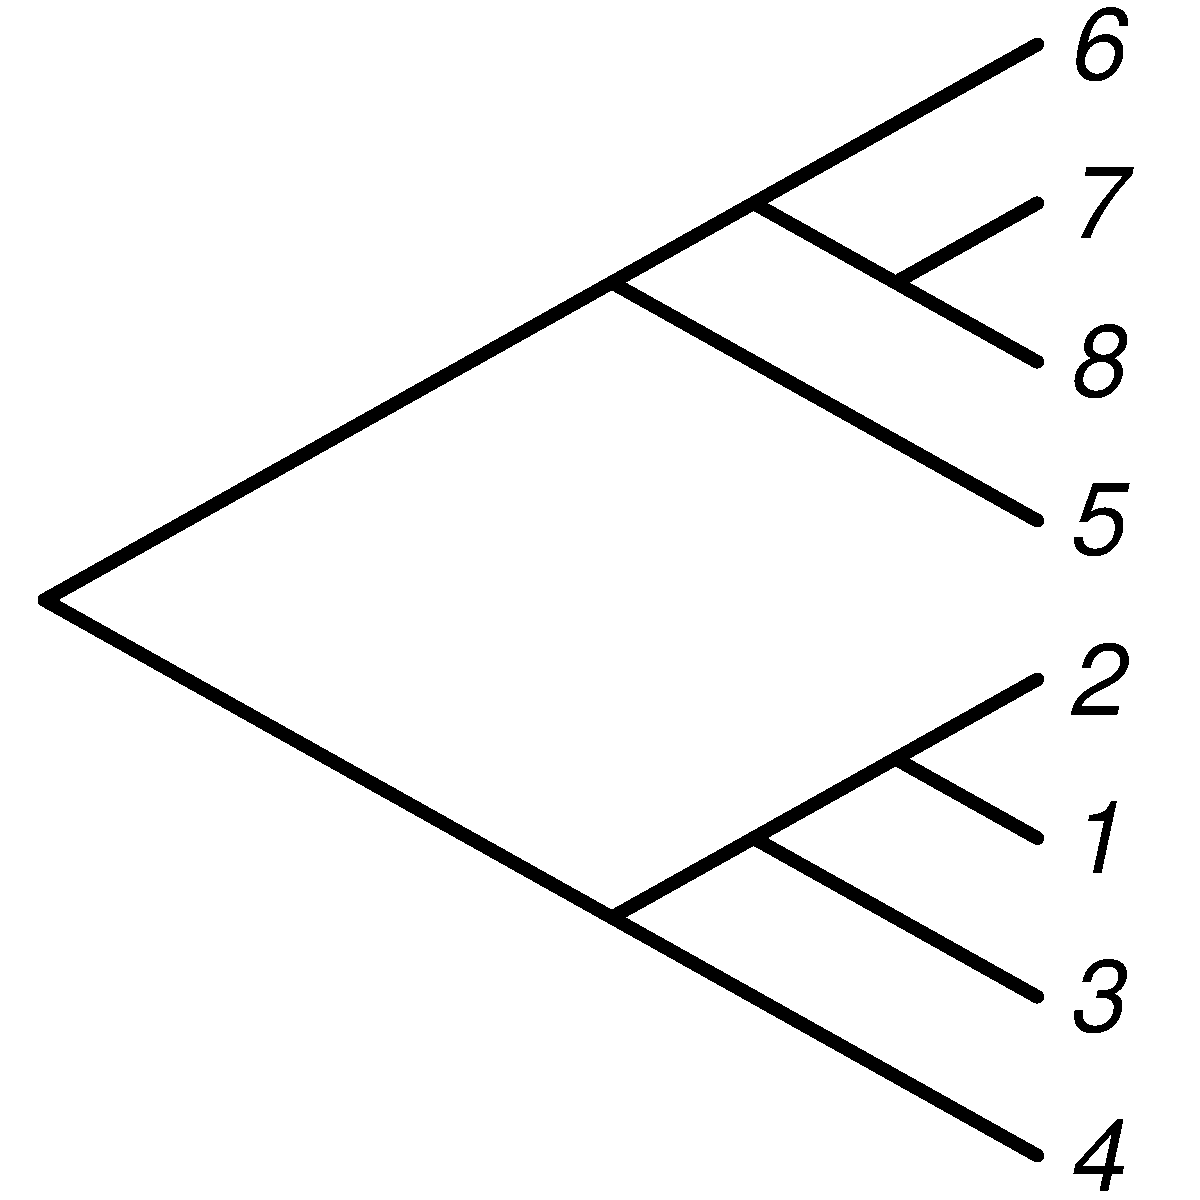
\includegraphics[width=.95\linewidth]{gatk_tree_rightwards.pdf}
% 	\end{block}
% 	\begin{block}{DiscoSNP++}
% 	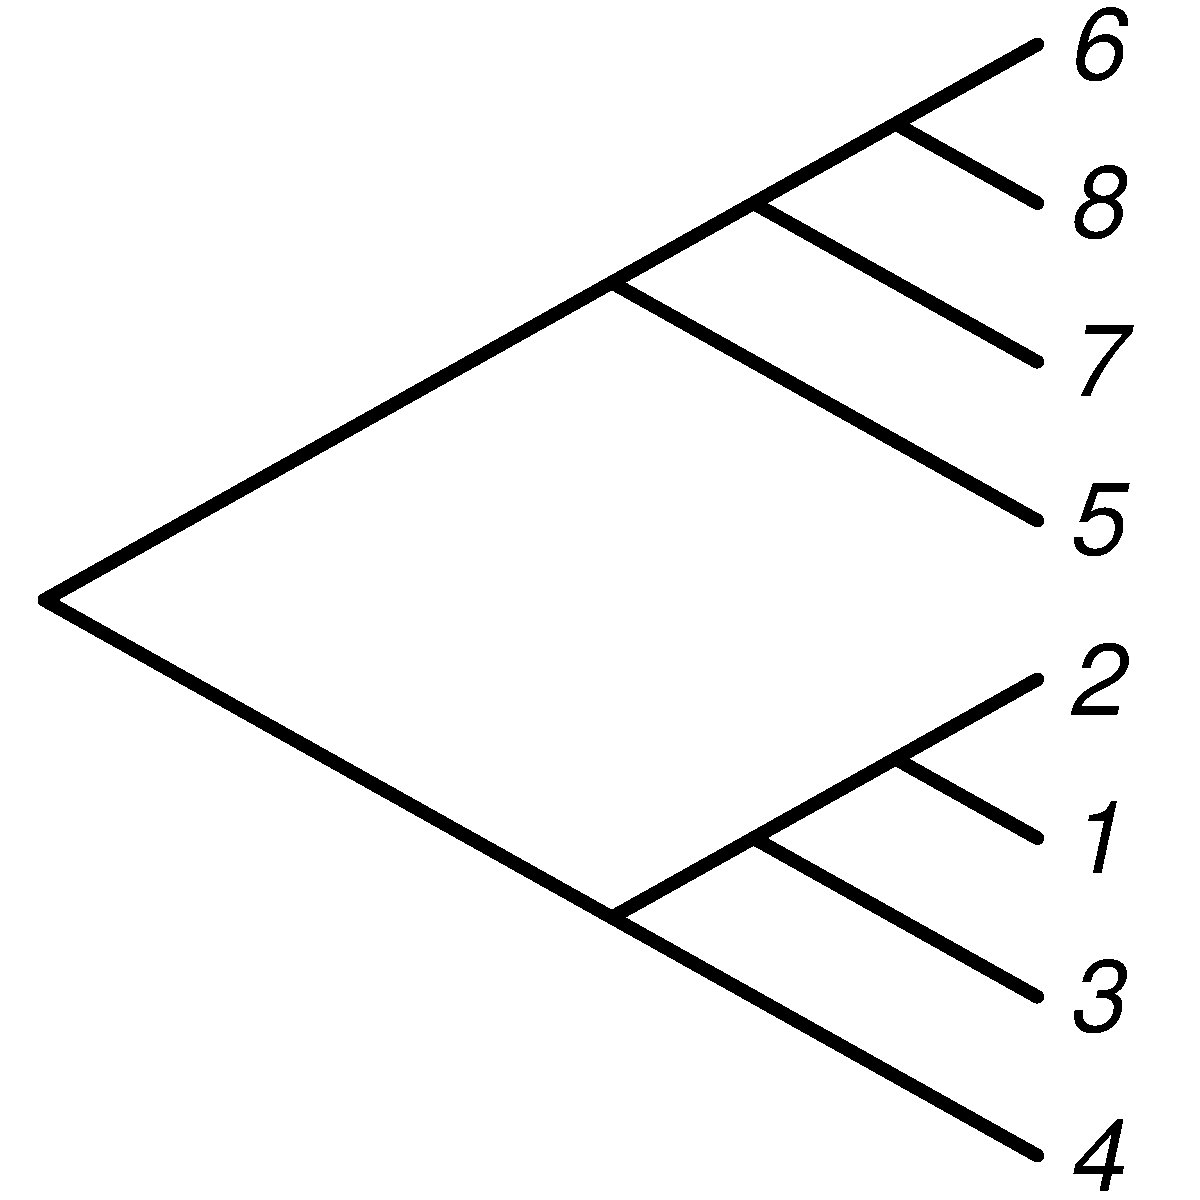
\includegraphics[width=.95\linewidth]{disco_tree_rightwards.pdf}
% 	\end{block}
% 	\column{.4\linewidth}
% 	\begin{block}{True Topology}
% 	\begin{center}
% 	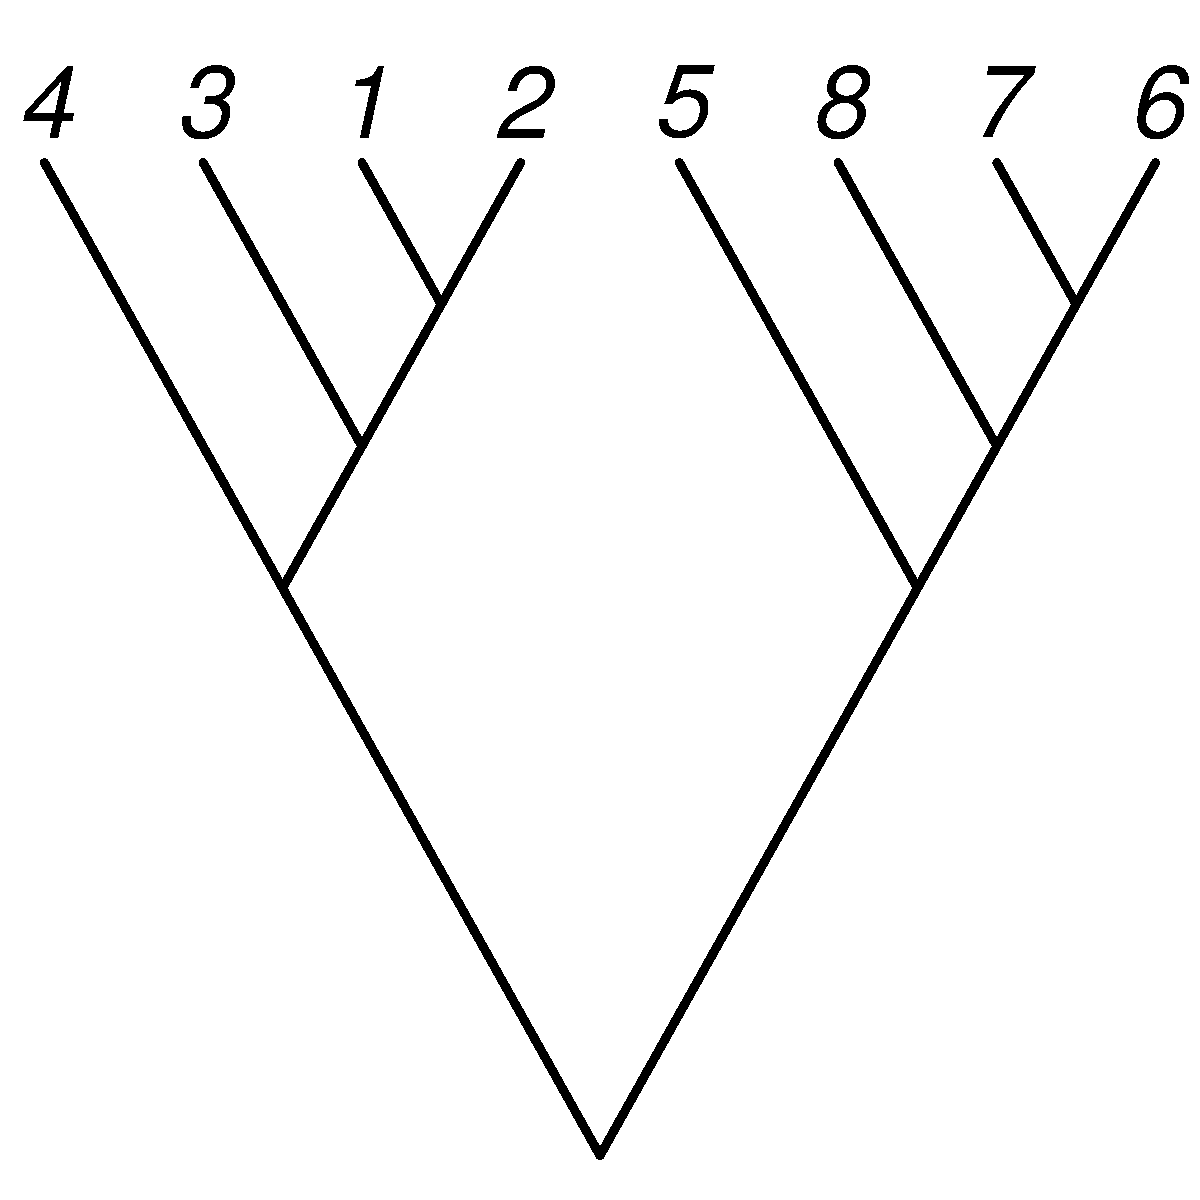
\includegraphics[width=.95\linewidth,angle=90]{true_tree.pdf}
% 	\vskip 1ex
% 	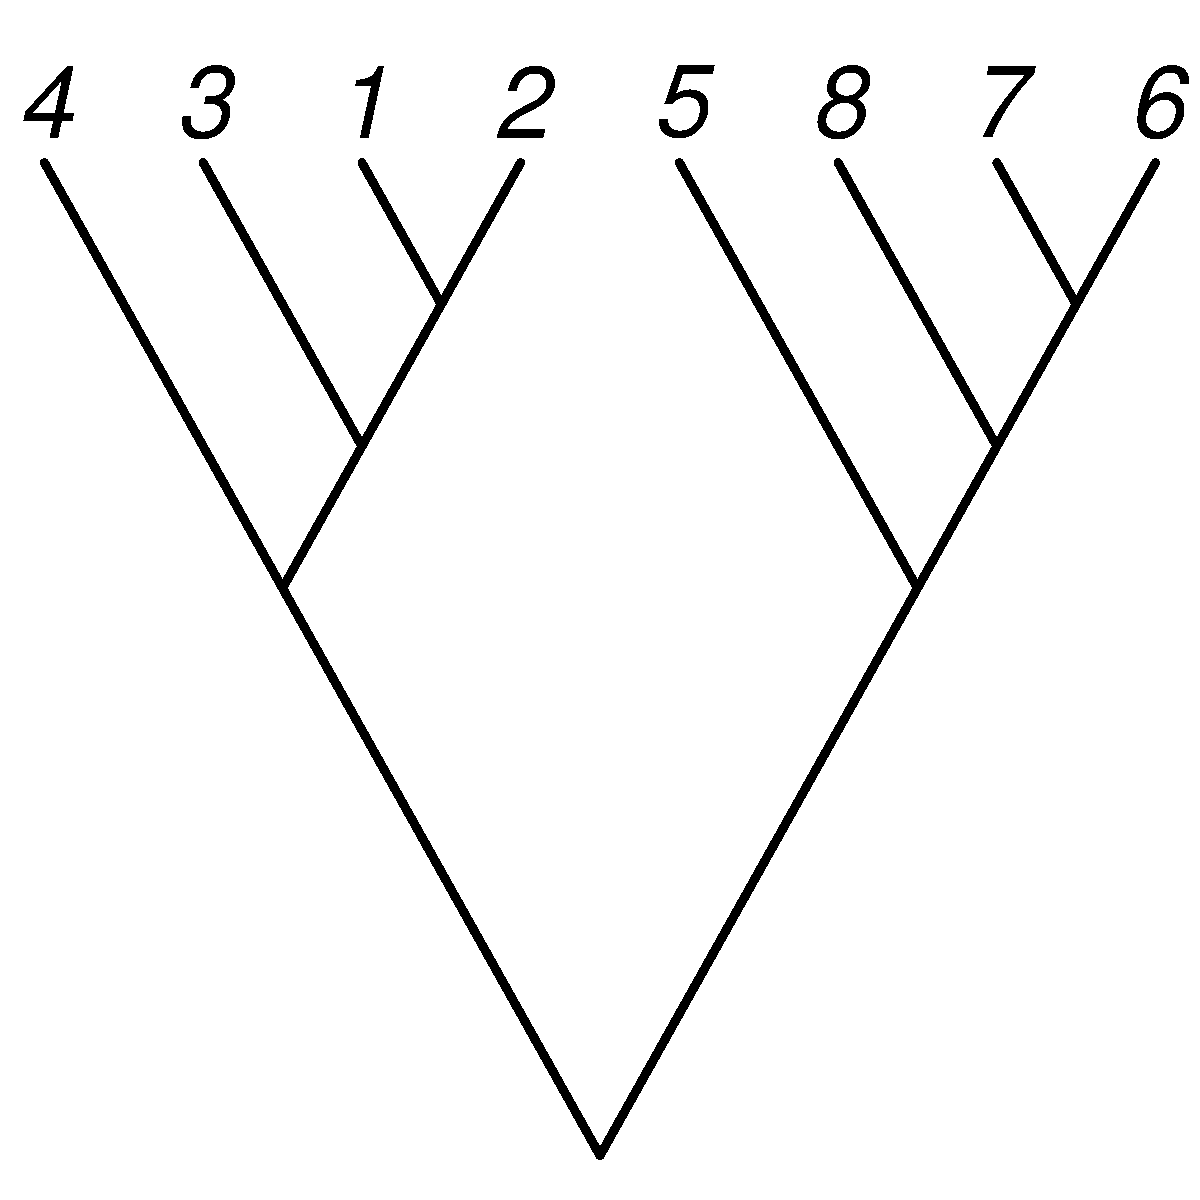
\includegraphics[width=.95\linewidth,angle=90]{true_tree.pdf}
% 	\end{center}
% 	\end{block}
% \end{columns}
\begin{center}
\begin{tabu} to .92\linewidth { X[-3,m] X[c,m] X[c,m] }
  & & True Topology \\
  & & \\
 GATK & 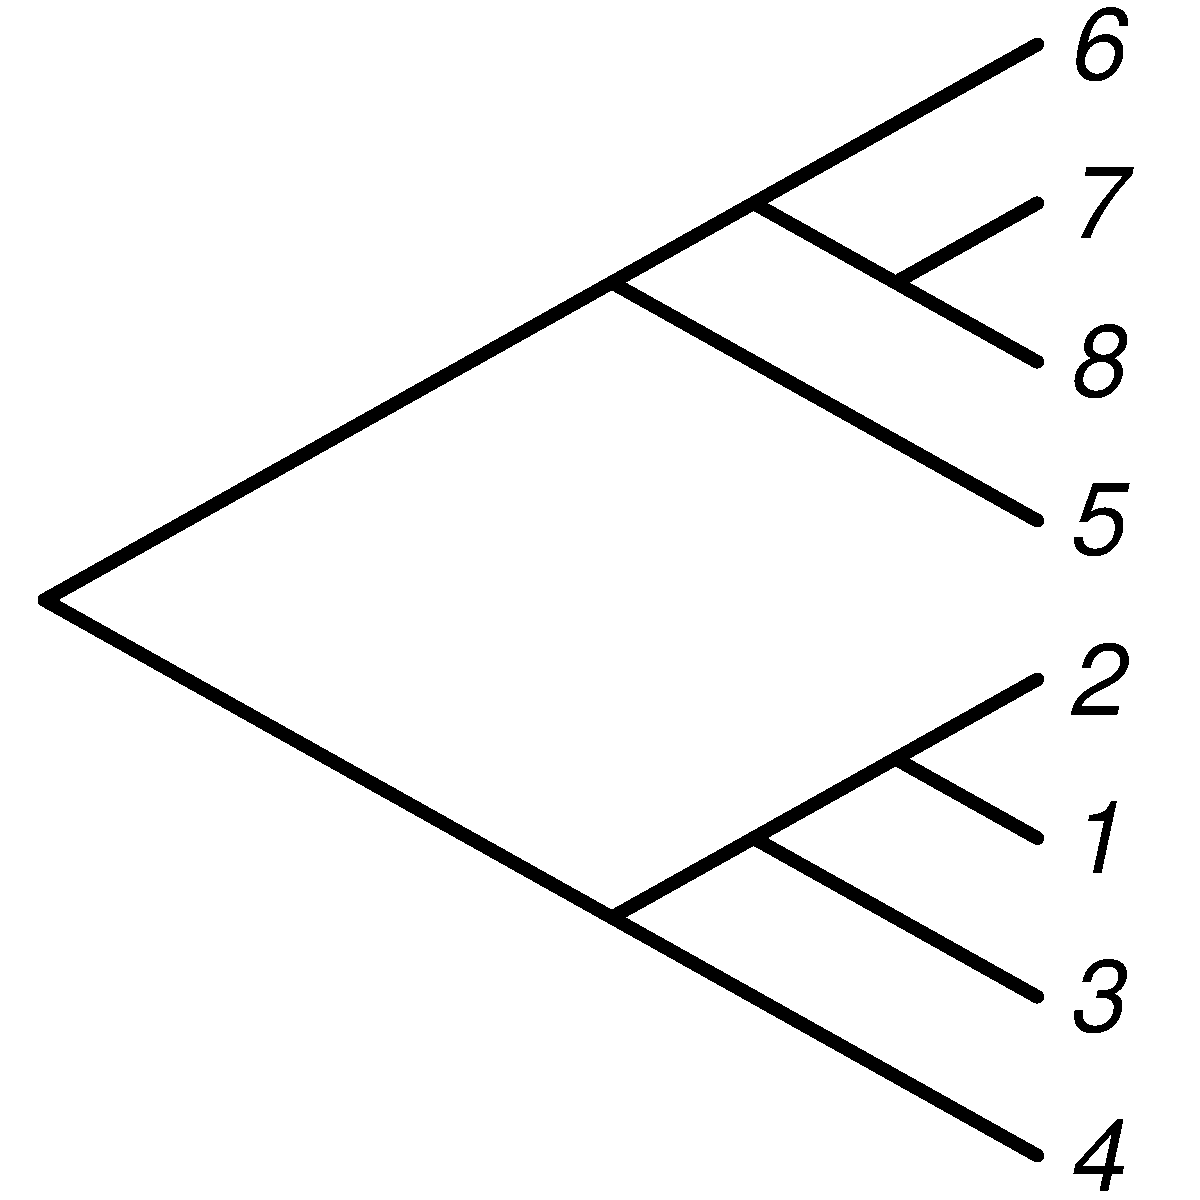
\includegraphics[width=.95\linewidth]{gatk_tree_rightwards.pdf} & 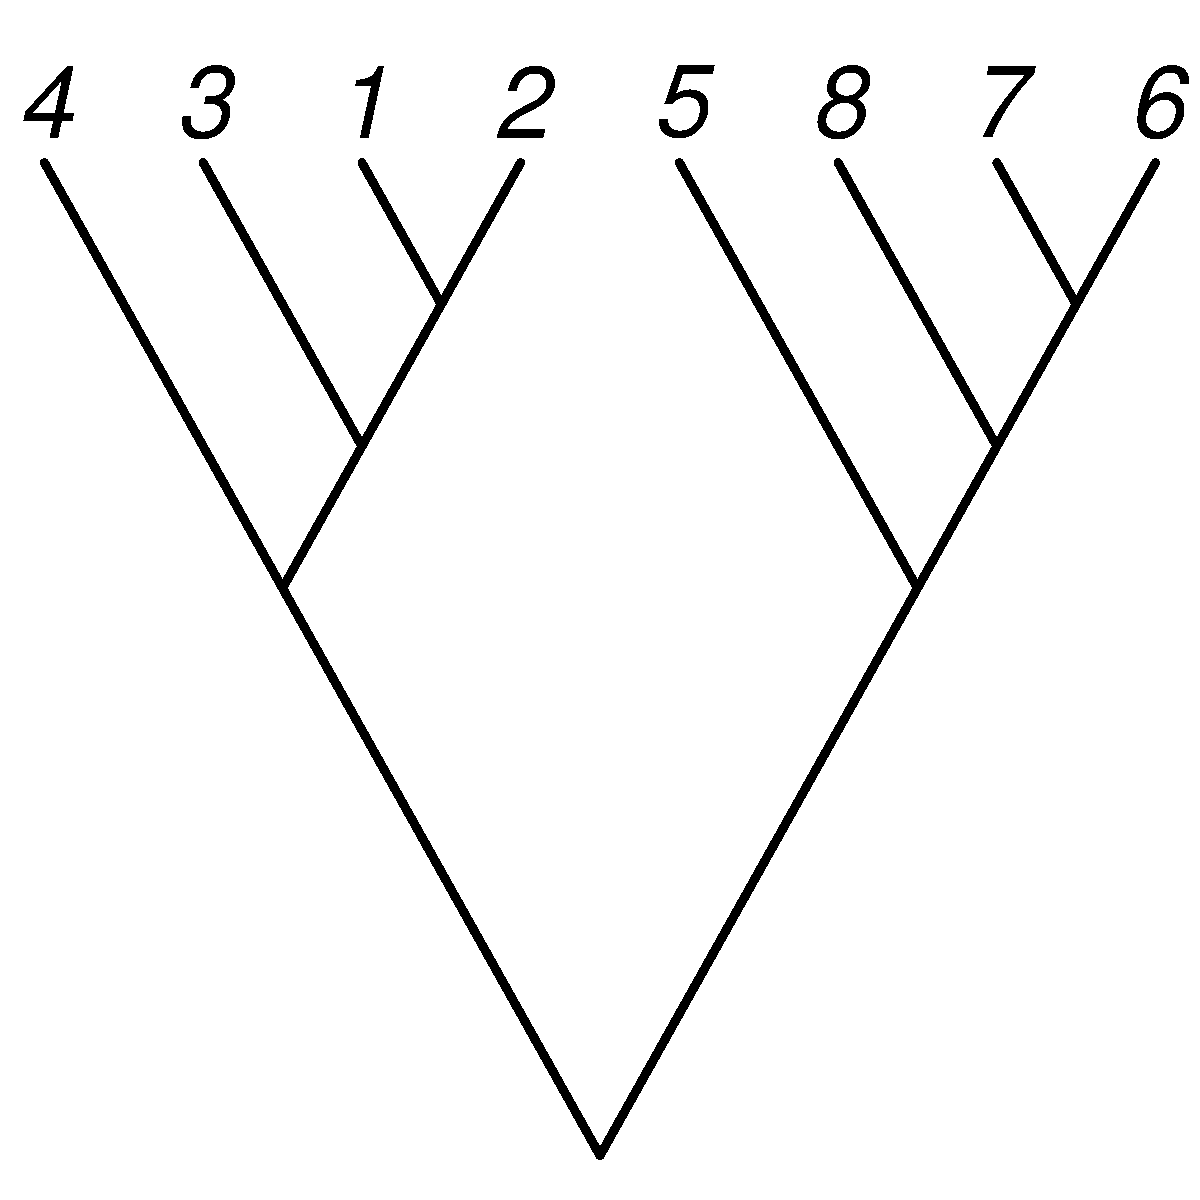
\includegraphics[width=.95\linewidth,angle=90]{true_tree.pdf} \\
  & & \\
 DiscoSNP++ & 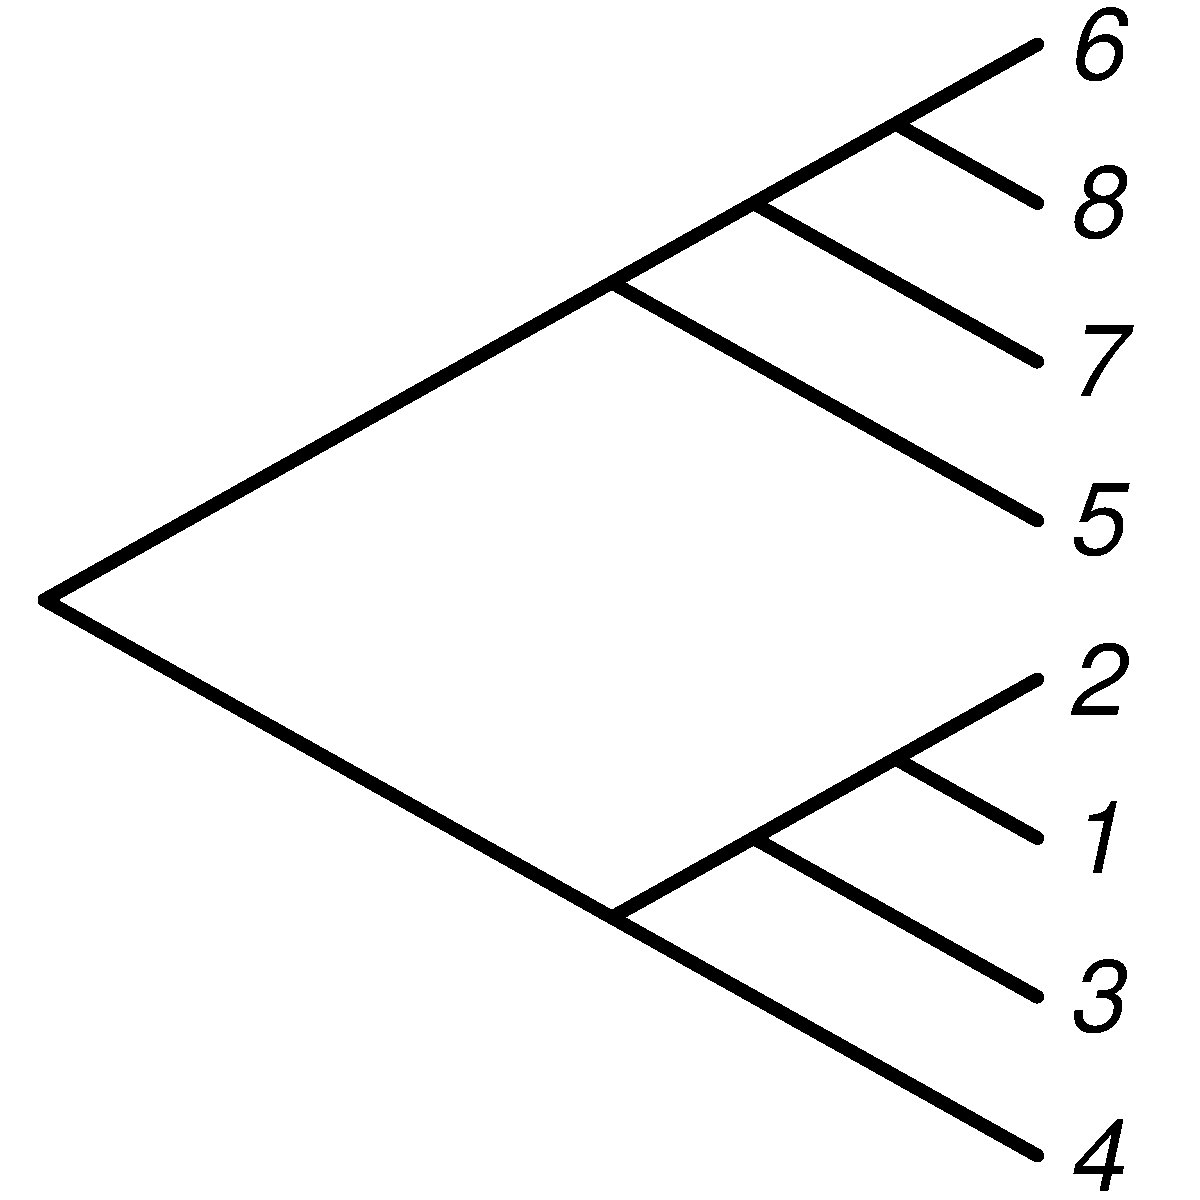
\includegraphics[width=.95\linewidth]{disco_tree_rightwards.pdf} & 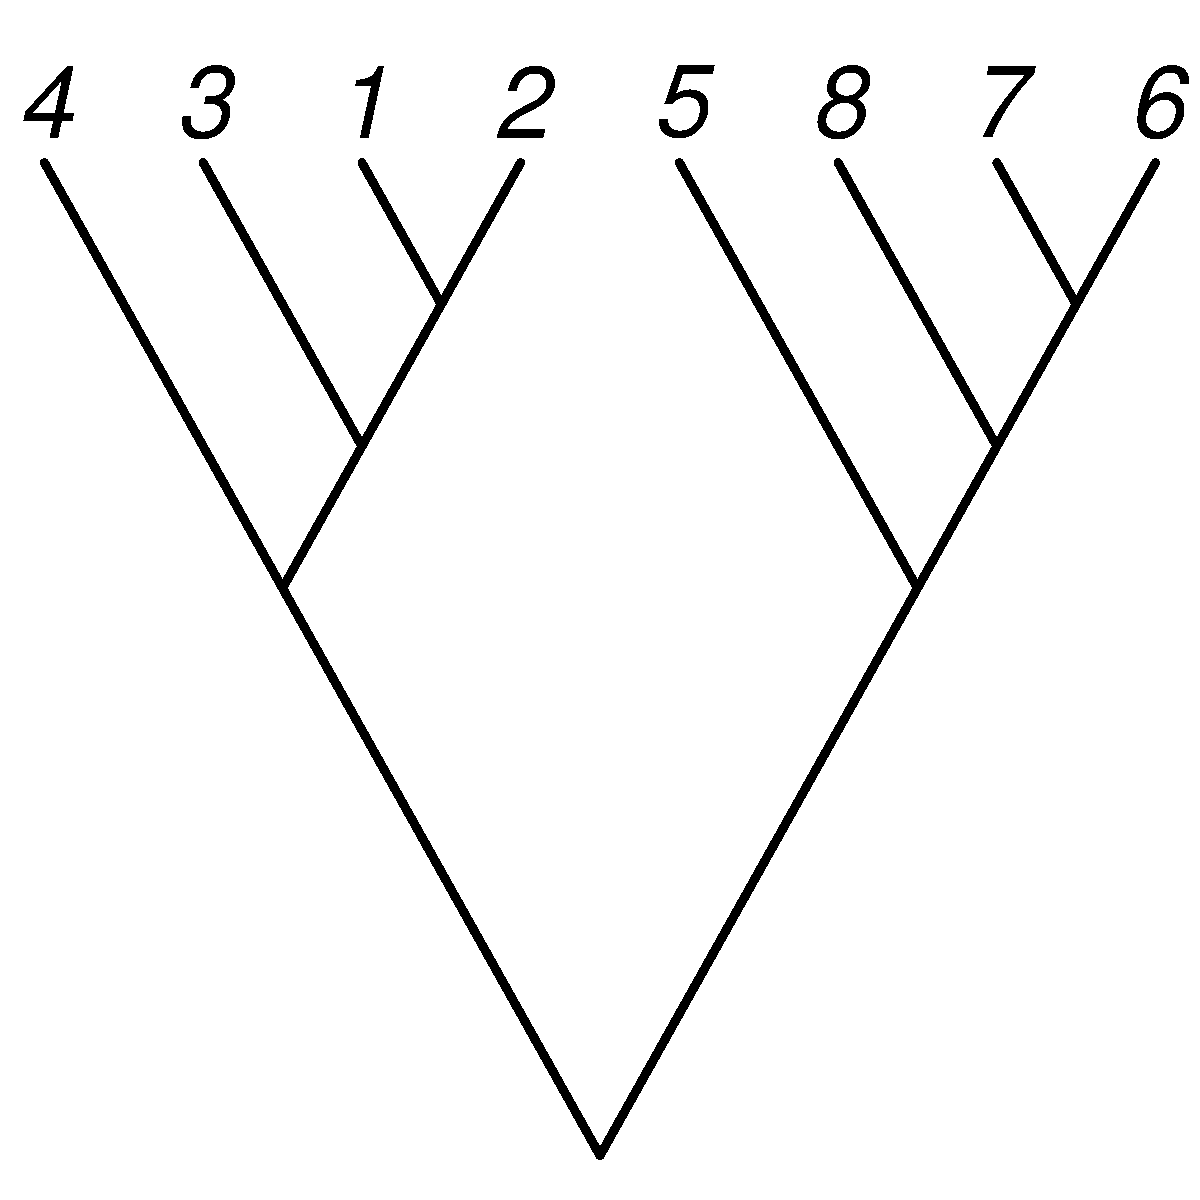
\includegraphics[width=.95\linewidth,angle=90]{true_tree.pdf}
\end{tabu}
\end{center}

% \vskip 3ex

% \begin{itemize}
% \item The toplogy of the tree built from variants called by reference-free method DiscoSNP++ closely resembles the branching pattern of the plant.
% \vskip 1ex
% \item DiscoSNP++ performance matches that of GATK used with a reference from the closely-related species \textit{Eucalyptus grandis}.
% \vskip 1ex
% \item A short internode causes incorrect placement of branches 6, 7, and 8 for both methods.
% \end{itemize}

\end{block}



%%% Right Side %%%%

\column{.5\linewidth}

%%%%%%%%%%%%%%%%%%%

\begin{block}{Next steps: Reference Improvement}

We improve our reference by aligning to the \textit{E. grandis} genome, then creating a consensus from that alignment. This can be repeated until convergence.

\vskip 1ex

\begin{center}
	\begin{tikzpicture}[cnode/.style={rectangle,draw=black!60,fill=black!5,very thick}, node distance = 3 cm]
		\node[cnode] (reads){Reads};
		\node[cnode] (eg)[below = .5cm of reads]{\textit{E. grandis}};
		\node[cnode] (em1)[right = of eg]{\textit{E. melliodora} 1};
		\node[cnode] (em2)[right = of em1]{\textit{E. melliodora} 2};
		\node[cnode] (etc)[right = of em2] {...};
		\draw[line width=3mm,->] ($(reads.east)-(0cm,.5cm)$) -- ($(reads.east)+(2cm,-.5cm)$) |- (em1.west);
		\draw[line width=3mm,->] (reads.east) -- ($(reads.east)+(13cm,0cm)$) |- (em2.west);
		\draw[line width=3mm,->] ($(reads.east)+(0cm,.5cm)$) -- ($(reads.east)+(24cm,.5cm)$) |- (etc.west);
		\draw[line width=3mm,->] (eg) -- (em1);
		\draw[line width=3mm,->] (em1) -- (em2);
		\draw[line width=3mm,->] (em2) -- (etc);
	\end{tikzpicture}
\end{center}

\end{block}


\begin{block}{Results: Iterative Mapping Improves Reference}

\begin{center}
	\begin{tikzpicture}[align=center,cnode/.style={rectangle,draw=black!60,fill=black!5,very thick}, node distance = .5cm and 2.5 cm]
		\node[cnode] (reads){Reads};
		\node[cnode] (eg)[below = of reads]{\textit{E. grandis}};
		\node[cnode] (em1)[right = of eg]{\textit{E. melliodora} 1};
		\node[cnode] (em1q)[right = of em1]{Alignment Quality Scores};
		\node[cnode] (egq)[below = of em1q]{Alignment Quality Scores};
		\draw[line width=3mm,->] ($(reads.east)-(0cm,.25cm)$) -- ($(reads.east)+(1.5cm,-.25cm)$) |- (em1.west);
		\draw[line width=3mm,->] ($(eg.east)+(1.25cm,0cm)$) -- ($(eg.east)+(1.25cm,-1cm)$) |- (egq.west);
		\draw[line width=3mm,->] (eg) -- (em1);
		\draw[line width=3mm,->] (em1) -- (em1q);
		\draw[line width=3mm,->] ($(reads.east)+(0cm,.25cm)$) -- ($(reads.east)+(12.5cm,.25cm)$) |- (em1q.west);
	\end{tikzpicture}
\end{center}

\vskip 1ex

\begin{center}

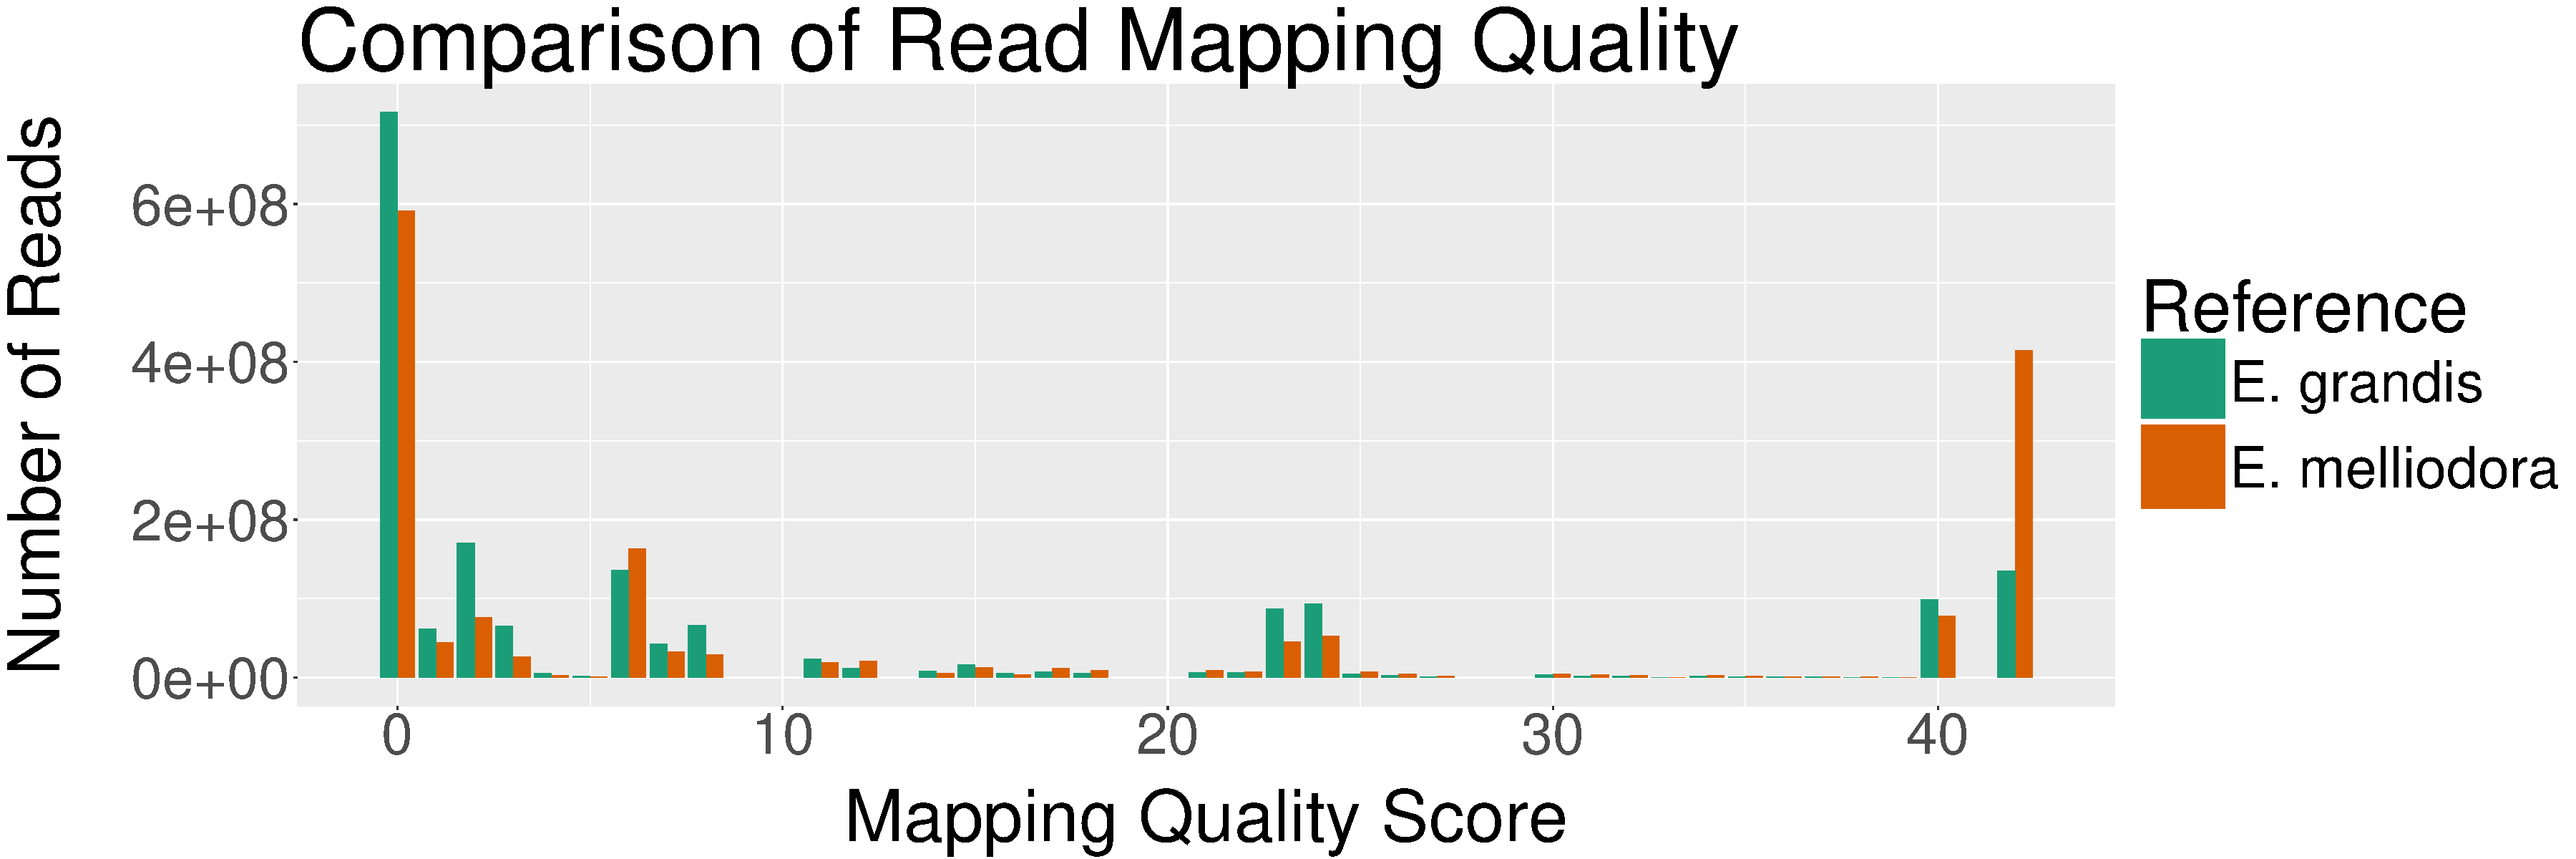
\includegraphics[width=.95\linewidth]{both_hist.pdf}

\end{center}

% \vskip 1ex

Alignment to the consensus sequence produces an alignment with higher overall quality scores than alignment to the \textit{Eucalyptus grandis} reference.

\end{block}


\begin{block}{Results: Aligner Choice Affects Generated Reference Quality}

\begin{center}
	\begin{tikzpicture}[align=center,cnode/.style={rectangle,draw=black!60,fill=black!5,very thick}, node distance = 2cm and 2cm]
		\node[cnode] (eg){\textit{E. grandis}};
		\node[cnode,minimum width=11cm] (reads)[right = of eg]{Reads};
		\node[cnode] (em1)[above right = 2cm and 4cm of eg]{\textit{E. melliodora} 1};
		\node[cnode] (em2)[below right = 2cm and 4cm of eg]{\textit{E. melliodora} 1};
		\node[cnode] (bwaq)[right = 4cm of em1]{Quality Scores};
		\node[cnode] (ngmq)[right = 4cm of em2]{Quality Scores};
		\draw[line width=3mm,->] (eg.north) |- (em1);
		\draw[line width=3mm,->] (eg.south) |- (em2);
		% \draw[line width=3mm,->] ($(reads.west)+(0cm,.5cm)$) to[out=180,in=180] ($(em1.west)-(1.5cm,0cm)$) -- (em1.west);
		\draw[line width=3mm,->] ($(reads.west)+(0cm,.5cm)$) -- ++(-1cm,0cm) |- (em1.west) node[pos=.25,right]{BWA};
		\draw[line width=3mm,->] ($(reads.west)-(0cm,.5cm)$) -- ++(-1cm,0cm) |- (em2.west) node[pos=.25,right]{NGM};
		\draw[line width=3mm,->] (em1) -- (bwaq);
		\draw[line width=3mm,->] (em2) -- (ngmq);
		\draw[line width=3mm,->] ($(reads.east)+(0cm,.5cm)$) -- ++(1cm,0cm) |- (bwaq.west) node[pos=.2,right]{Bowtie};
		\draw[line width=3mm,->] ($(reads.east)-(0cm,.5cm)$) -- ++(1cm,0cm) |- (ngmq.west) node[pos=.2,right]{Bowtie};
	\end{tikzpicture}
\end{center}

\vskip 1ex

\begin{center}

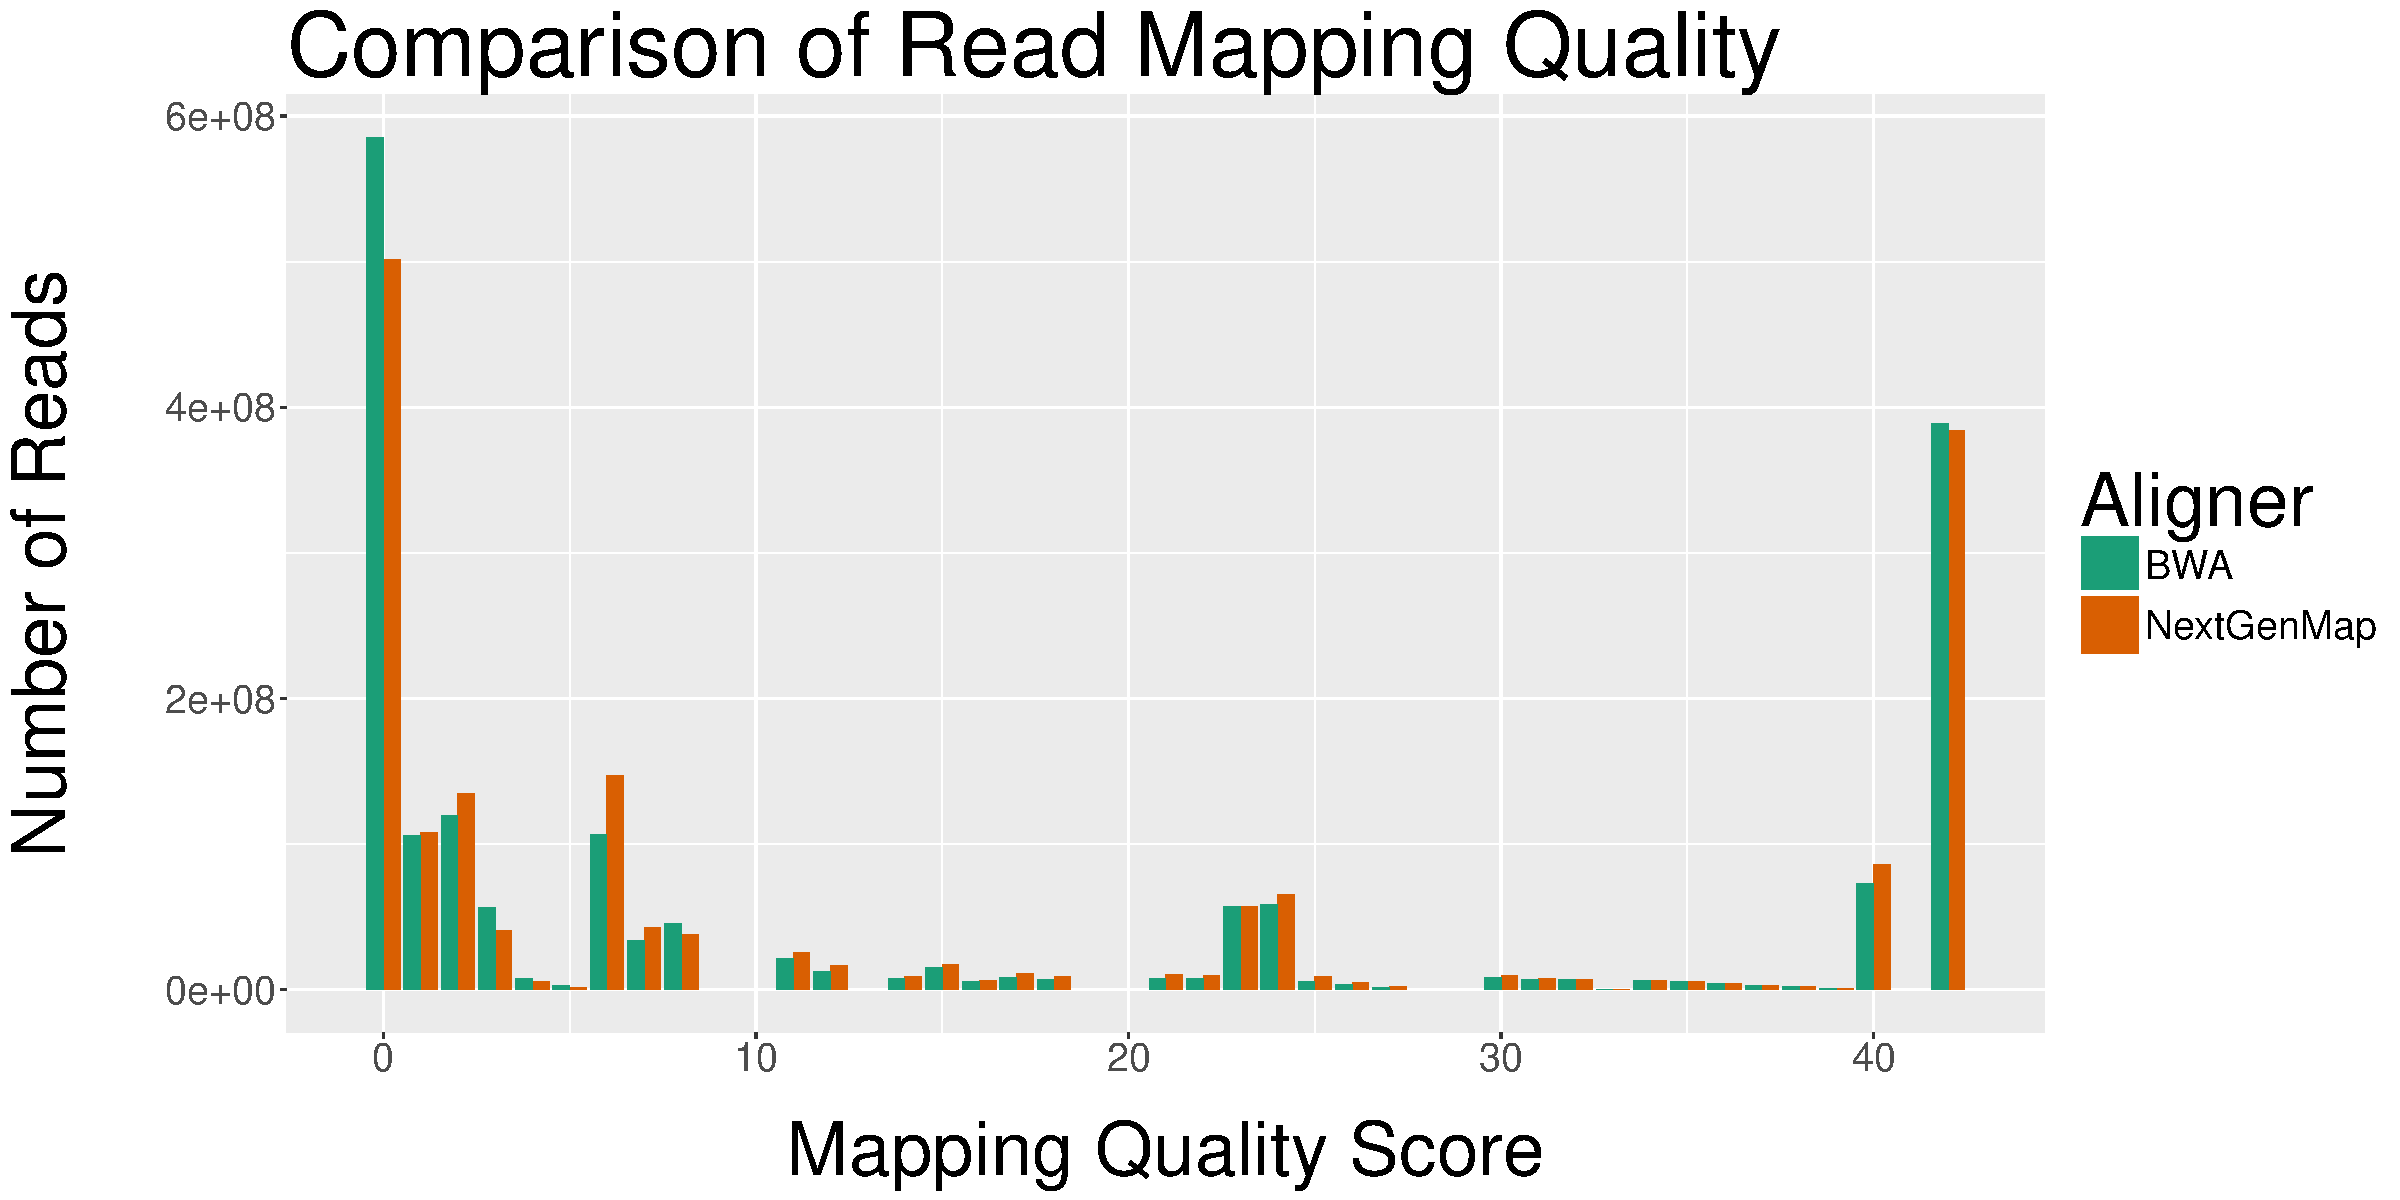
\includegraphics[width=.95\linewidth]{aligner_comparison_hist.pdf}

\end{center}

% \vskip 1ex

% A reference created from a NextGenMap alignment produces less unmapped reads than one created from a BWA alignment.

\end{block}




\begin{block}{Conclusions}

\begin{itemize}
	\item Phylogenies of somatic mutations within a \textit{Eucalyptus} tree match the branching patterns of the tree using both a reference-based and a reference-free variant caller.
	\item Aligning reads to a close relative, obtaining a consensus sequence, then realigning to that consensus seems to improve alignment quality.
\end{itemize}

\end{block}


\begin{block}{Acknowledgements}

% \begin{center}

\begin{columns}
\column{.4\linewidth}
This work is supported by grants NIH R01-HG007178 and NSF DBI-1356548.
\column{.27\linewidth}

\includegraphics[width=\linewidth]{lab_logo.pdf}
\column{.27\linewidth}

\includegraphics[width=\linewidth]{sols_logo.pdf}
% \column{.2\linewidth}
% 
\includegraphics[width=\linewidth]{nih-nhgri-official-logo.jpg}
\end{columns}

% \end{center}

\end{block}

\end{columns}
\end{frame}

\end{document}